\documentclass{article}
\usepackage{comment}
\usepackage[english]{babel}
\usepackage[utf8]{inputenc}
\usepackage{fancyhdr}
\usepackage[round]{natbib}
\usepackage{graphicx}
\usepackage{url}
\usepackage{amsmath}
\DeclareMathOperator*{\argmax}{argmax}
\pagenumbering{arabic}

\pagestyle{fancy}
\fancyhf{}
\rhead{Mohammad Rahmani}
\lhead{The Nostalgia Factor}

\newcommand{\ignore}[1]{}
\begin{document}
	\bibliographystyle{plainnat}
	\title{The Computational Aspect of Nostalgia}
	\author{Mohammad Rahmani}
	\date{}
	\maketitle
	\section{Introduction}\label{sec:introduction}
	The idea is that a good story is a story which incorporates more semantic units (in this document semantic units exemplified as words, but as a future work this can be extended to events etc) in a shorter length. For example in Figure \ref{fig:boy-clock}, two objects are detected. A "clock" and a "boy". The question is, if we have two candidate narratives(as sequences of events) both of which contain both the terms \{click,boy\}, then, which of them is better. With regard to interestingness, according to an experiment carried out in \citet{mcintyre-2009-learning-to-tell-tales-a-data-driven-approach-to-story-generation} and described in its Section 2.4, narratives which introduce more objects(and relations) are supposed to be more interesting. A close translation to this conception might be the more a narrative, implicitly, reminds the reader of the objects which do not exist in a narrative, the better the story is. This notion, in psychology and art, is coined as \textit{nostalgia}. The rest of this paper suggests a computational approach toward developing an scale to measuring and comparing the intensity of nostalgia in different stories as one of the indexes that may drive a narrative to a more captivating state.  
	\begin{figure}[h!]
		\centering
		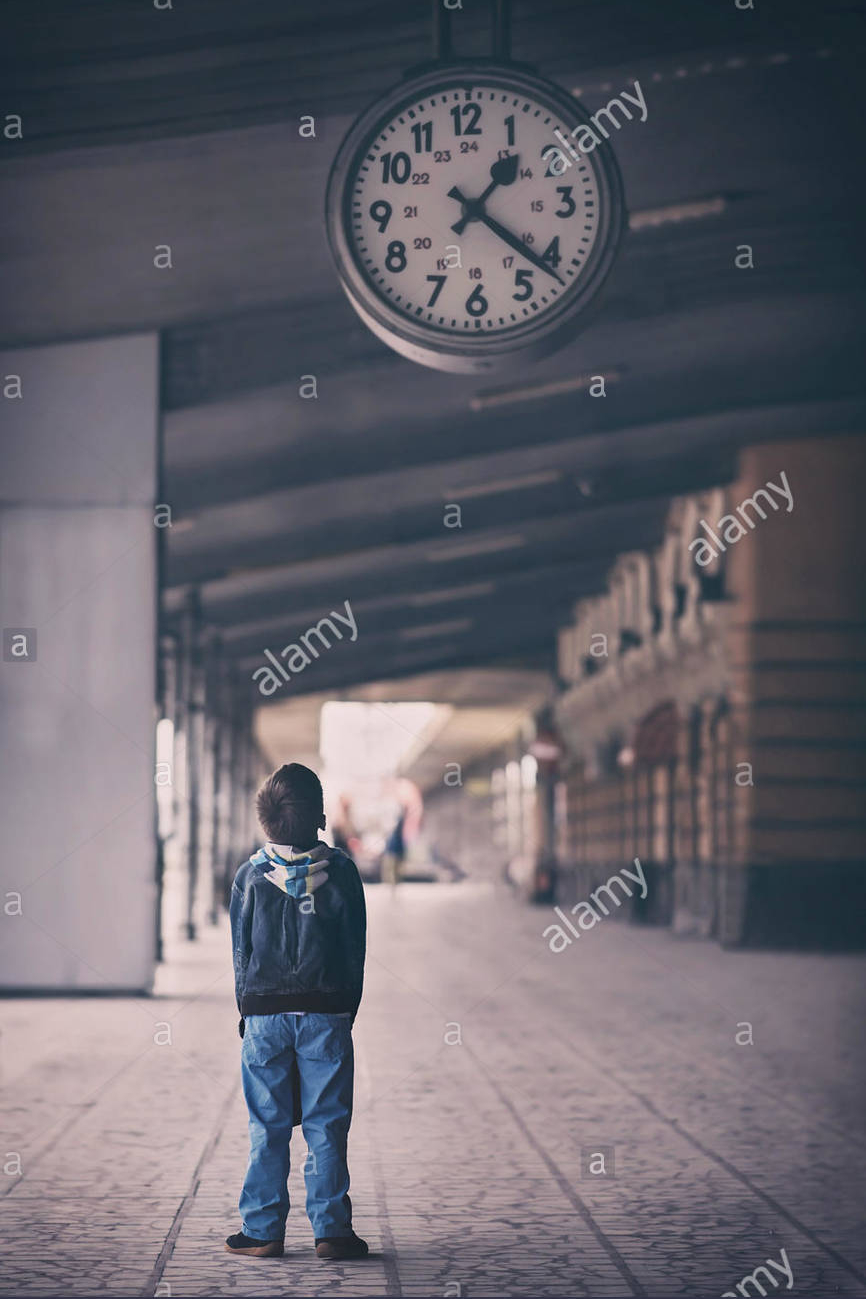
\includegraphics[width=0.5\textwidth]{/media/donkarlo/Elements/projs/research/assets/boy-clock.jpg}
		\caption{In this image S=\{clock,boy\} from which many narratives is crafted during training phase. A story is more nostalgic that its sequence of semantic units passes through a denser area in semantic vector space of all training narratives.} 
		\label{fig:boy-clock}
	\end{figure}
	\section{Methodology}
	We first need to build the vector semantic space for the dictionary of the words which have appeared in all the training narratives such as the solution suggested in \citet{m}. Lets say for a set of $k$ input semantic units(input words) such as 
	\begin{equation}
		S =\{s_1,...,s_{k}\}
	\end{equation}	
	some candidate narratives should be crafted (by an automatic narrative generator model) such that all of them contain all words in S. If N represents the set of candidate narratives which contains $|N|$ different narratives, then a typical member of it could be represented as follows:
	\begin{equation}
		N_i=\{\vec{s}_{i,1},...,\vec{s}_{i,|N_i|}\} \ni \forall i\in\{1,...,|N|\} , S \subset N_i
	\end{equation}
	where $|N_i|$ is the number of semantic units in narrative $N_i$. 
	
	If $C_i$ is taken as the union of the areas covered by the circles(spheres) formed around the constituent semantic unit vectors in $N_i$ as is described in Equation \ref{eq:neighborhood-semantics}
	\begin{equation}
		\cup C_i = \{|\vec{x}-\vec{s}_{i,j}|<{r_{i,j}}\}_{j=1}^{|N_i|} \ni i \in \{1,...,|N|\}
		\label{eq:neighborhood-semantics}
	\end{equation}
	such that 
	\begin{equation}
		\frac{\sum_{j=1}^{|N_i|}r_{i,j}}{|N_i|} = R
		\label{eq:radius-limit}
	\end{equation}
	then $C_i$ can be used as a basis to establish a scale to measure and compare the nostalgia rate in narratives. Literally, this  scale states a narrative is better if its semantic unit constituent neighborhoods cover a more crowded area of semantic units mentioned in all training narratives. R in \ref{eq:radius-limit} will be constant across all candidate narratives. It could be regarded as nostalgic memory domain radius. The rationality for establishing the restriction formulated in Equation \ref{eq:radius-limit} is that in case we increase the radius for the circle around one constituent semantic unit of a narrative, then it entails decreasing the radius of other circles accordingly. As such, fairness across all the candidate narratives will be maintained while we will have the opportunity to extend search radius around a particular semantic unit. The denominator guarantees that a lengthier narrative is not necessarily a better one. Finally if $W_i$ is the set of semantic units which exist in cloud $C_i$ and $|W_i|$ is its corresponding members' number, then the best narrative is: 
	\begin{equation}
	\argmax_{i=1}^{|N|} \frac{|W_i|}{|N_i|}
	\label{eq:argmax}
	\end{equation}
	Figure \ref{fig:clouds-around-two-candidate-stories} exemplifies all the aforementioned subjects into a single illustration with a detailed explanation in its caption.  
	\begin{figure}[h!]
		\centering
		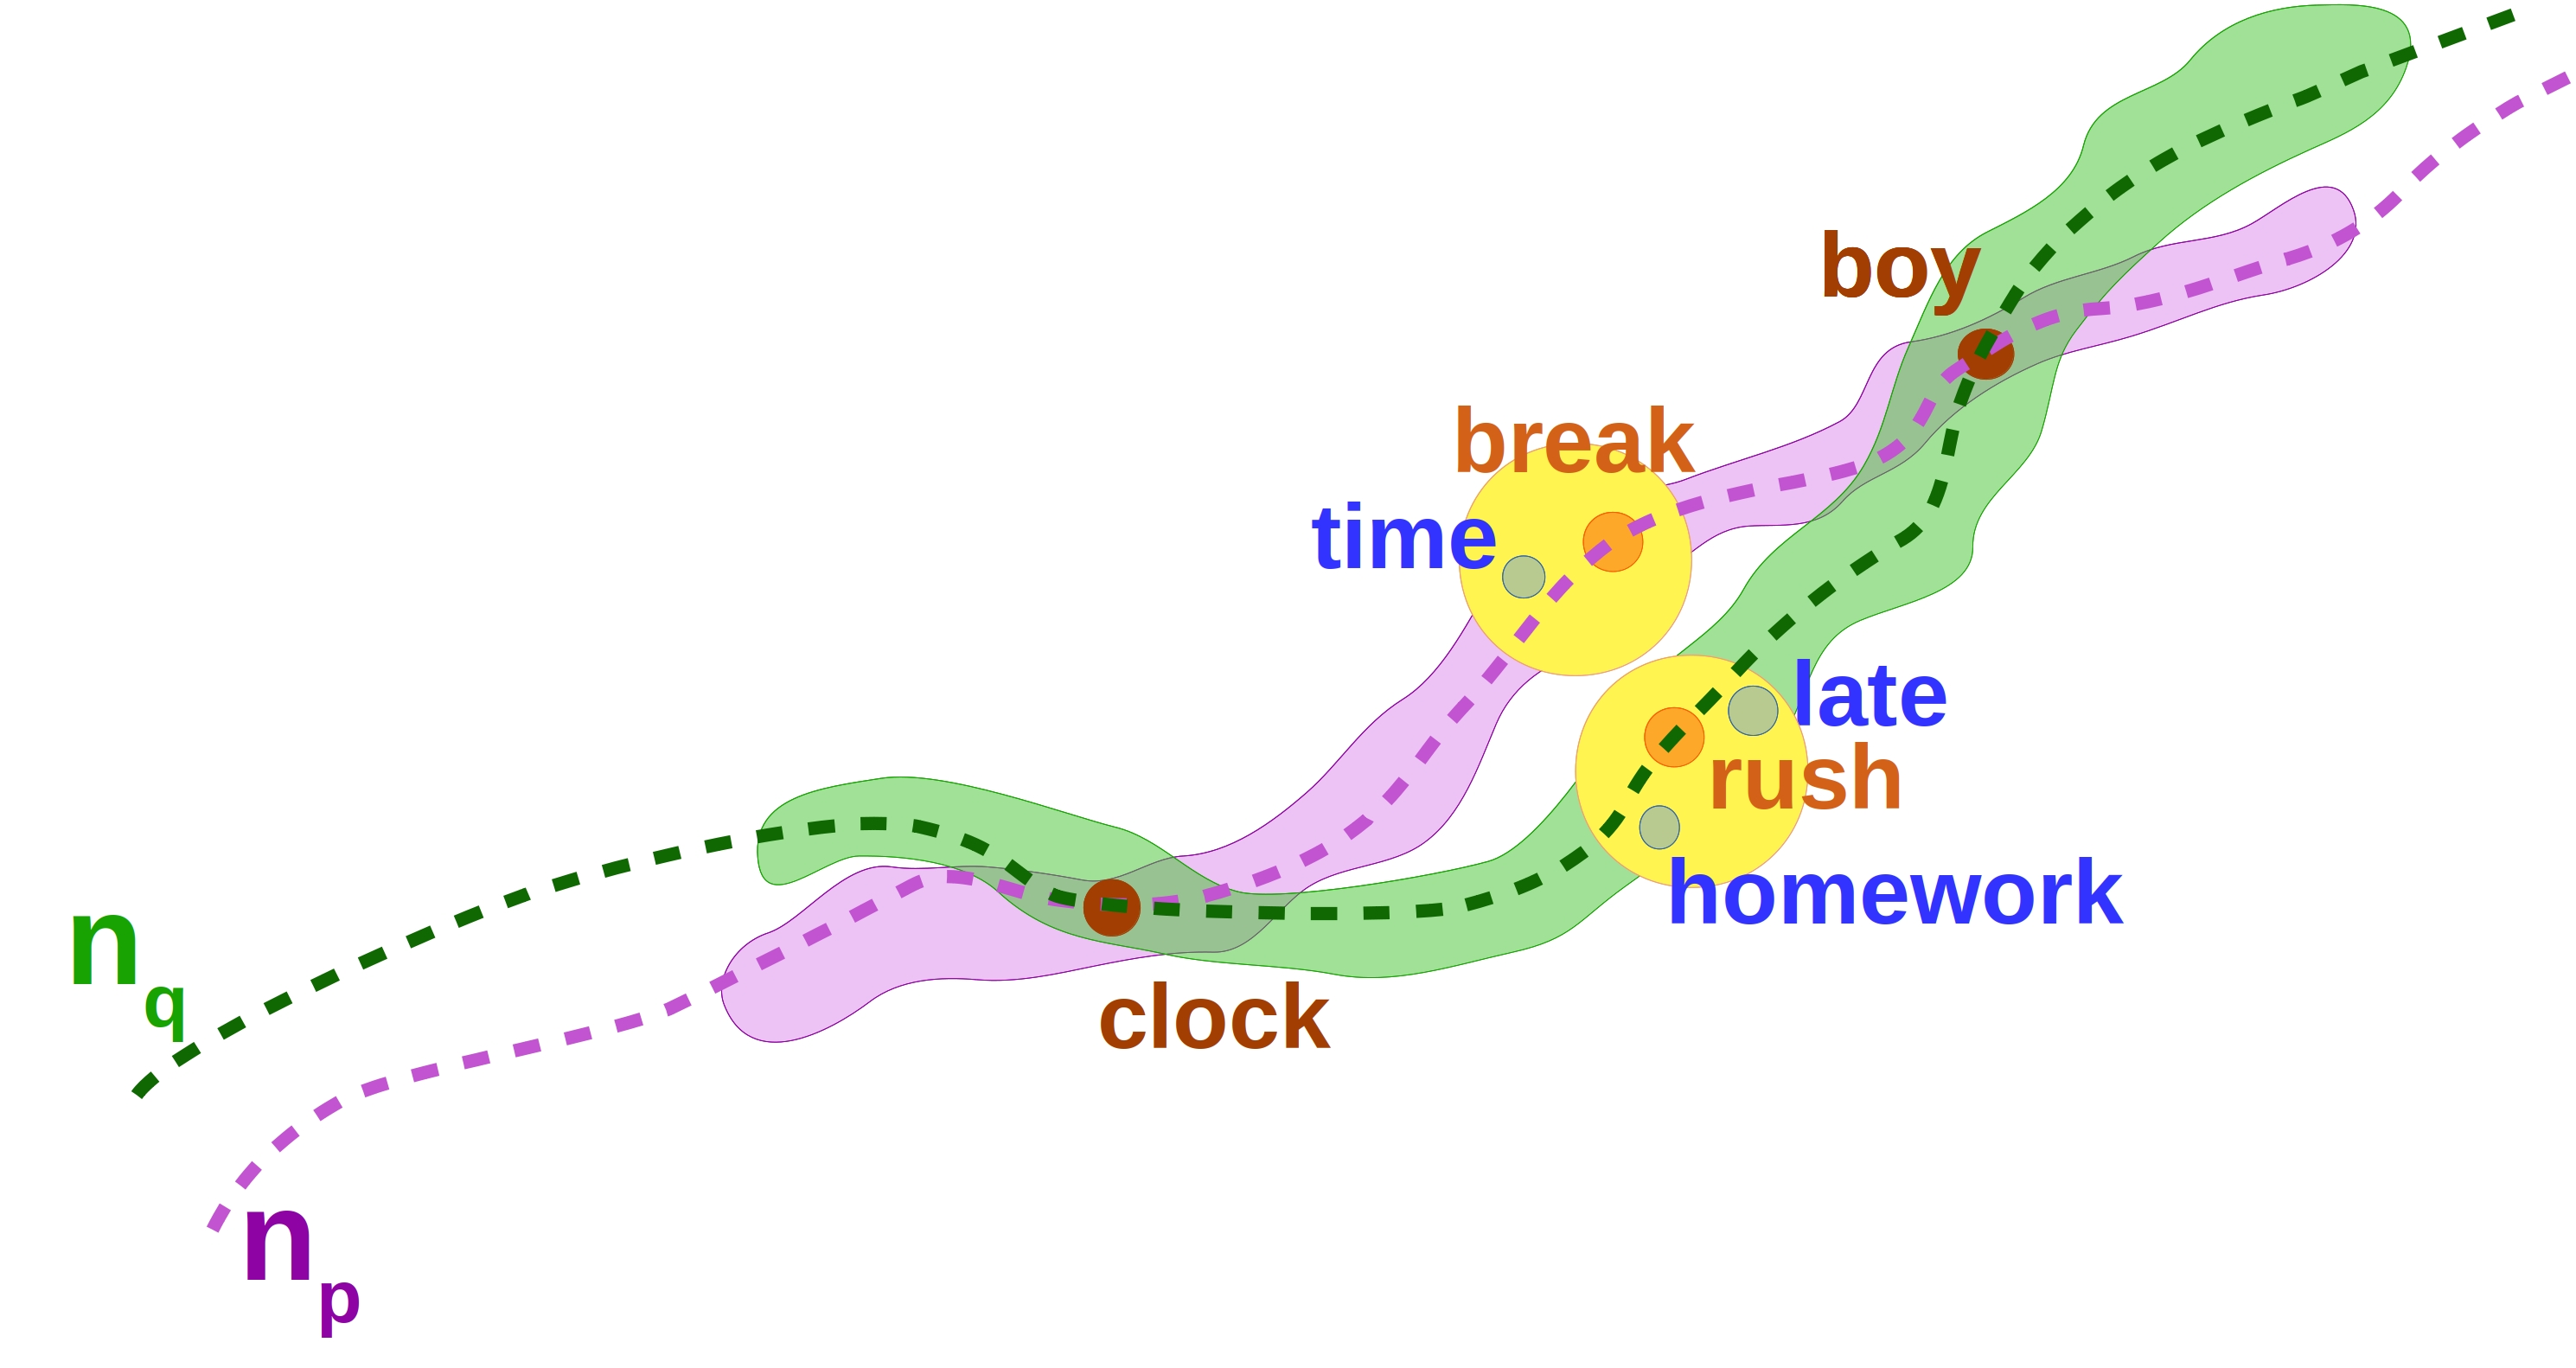
\includegraphics[width=1\textwidth]{/media/donkarlo/Elements/projs/research/assets/cloud-evaluation.jpg}
		\caption{In this figure, $S=\{clock,boy\}$ is the set for which the narrative generator model should generate several candidate narratives. Lets say the model has generated two candidate narratives such as $N=\{n_q,n_p\}$ in which $n_q$="The \textbf{boy} looked at the \textbf{clock} and found that he has to \textbf{rush}" and $n_p$="The \textbf{clock} reminded the \textbf{boy} of a \textbf{break}". In other words $n_q=\{clock,rush,boy\}$ and $n_p=\{clock,break,boy\}$. The cloud around ${rush} \in n_q$ contains the semantic units $\{late,homework\}$ and the cloud around $"break" \in n_p$ contains $\{time\}$. Both these sets are formed of training narratives other than $n_p$ and $n_q$. Since $|n_q|=|n_s|=3$ then according to Equation \ref{eq:argmax}, $n_q$ is a better story(more nostalgic). Subjectively, it is more intresting because it may remind the reader a of rushing to do his/her homework when s/he was young for not being late!} 
		\label{fig:clouds-around-two-candidate-stories}
	\end{figure}
	\bibliography{/media/donkarlo/Elements/projs/research/refs}
\end{document}